\documentclass[a4paper,10pt]{article}

\usepackage{ucs}
\usepackage[utf8]{inputenc}
\usepackage{amsmath}
\usepackage{amssymb}
\usepackage[english]{babel}
\usepackage[T1]{fontenc}
\usepackage[pdftex]{graphicx}
\usepackage{xspace}
\usepackage[pdftex]{hyperref}

\author{E. Chapon}
\title{Notes on quarkonium scaling}
\date{06/11/2017}

\newcommand{\Jpsi}{\ensuremath{\text{J}/\psi}\xspace}
\newcommand{\xt}{\ensuremath{x_T}\xspace}
\newcommand{\pt}{\ensuremath{p_T}\xspace}
\newcommand{\mt}{\ensuremath{m_T}\xspace}
\newcommand{\sqrts}{\ensuremath{\sqrt{s}}\xspace}
\newcommand{\dd}{\ensuremath{\text{d}}\xspace}

\begin{document}
 \section{Code}
 It is available in git: \url{https://github.com/echapon/scalingOnia}.

 \section{Scaling variable}
 
 Two scaling variables are considered:
 
 \begin{equation}
  \xt^1 = \frac{2 \times \pt}{\sqrts}~\cite{xt}
 \end{equation}
 
 and
 
 \begin{equation}
  \xt^2 = \frac{\pt + \mt}{\sqrts} = \frac{\pt + \sqrt{\pt + m_{\Jpsi}}}{\sqrts}
 \end{equation}
 
 \section{Determination of the effective $n^\text{eff}$ exponent}
 
 The first step is to plot the cross section as a function of \xt instead of \pt. For this we simply plot $\dd \sigma / \dd \xt = \dd \sigma / \dd \pt \cdot \left(\dd \xt / \dd \pt\right)^{-1}$ as a function of \xt, following one of the definitions described above.
 
 Then we use the fact that we expect a scaling of the form 
 
 \begin{equation}
  \frac{\dd \sigma}{\dd \pt} \propto \frac{F(\xt)}{\pt^n}
 \end{equation}

 to extract the effective exponent as a function of \xt:
 
 \begin{equation}
  n^\text{eff} (\xt) \equiv - \frac{\ln \left(\frac{\dd \sigma}{\dd \pt}(\xt, \sqrt{s_1}) / \frac{\dd \sigma}{\dd \pt}(\xt, \sqrt{s_2}) \right)}{\ln\left(\sqrt{s_1}/\sqrt{s_2}\right)}
 \end{equation}

 
 \section{Interpolation}
 Because we need to compare the data (or the theory) at fixed \xt, we need to interpolate between two data points. This interpolation can be done in several ways. Four interpolations
 are implemented:
 
 \begin{itemize}
  \item linear interpolation;
  \item cubic spline interpolation (locally cubic and ensuring continuity of the first and second derivatives);
  \item linear in log-log space (default because naturally corresponds to the assumption of a locally power-law spectrum);
  \item cubic spline in log-log space.
 \end{itemize}
 
 \subsection{Interpolation and uncertainties}
 
 \begin{figure}
  \begin{center}
   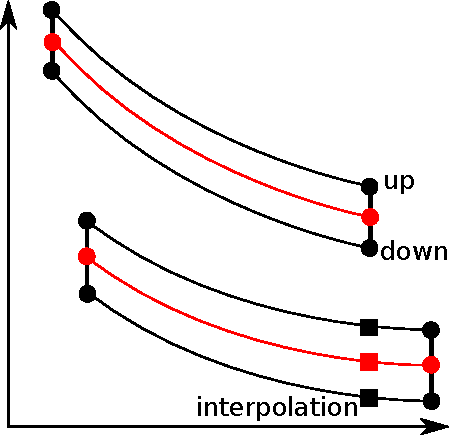
\includegraphics[width=0.5\textwidth]{uncert_interpol.pdf}
  \end{center}
  \caption{Propagation of the uncertainties in the ratio, involving interpolation.
  \label{fig:uncert_interpol}}
 \end{figure}

 When using the interpolation for computing the ratio of two graphs (sets of points), the uncertainties also have to be properly propagated. The procedure used is illustrated in Fig.~\ref{fig:uncert_interpol}.
 The upper and lower limits of the uncertainty band are interpolated in the same way as the central values. Then the uncertainty is propagated with standard error propagation.
 
 \paragraph{Ratio of cross sections}
 
 \begin{eqnarray}
  R & \equiv & \frac{\dd \sigma_\text{num} / \dd \pt}{\dd \sigma_\text{den} \dd \pt}\\
  \dd^\text{up} R & = & R \times \sqrt{(\dd^\text{up} \left(\dd \sigma_\text{num}/\dd\pt\right))^2 + (\dd^\text{down} \left(\dd \sigma_\text{den}/\dd\pt\right))^2} \\
  \dd^\text{down} R & = & R \times \sqrt{(\dd^\text{down} \left(\dd \sigma_\text{num}/\dd\pt\right))^2 + (\dd^\text{up} \left(\dd \sigma_\text{den}/\dd\pt\right))^2}
 \end{eqnarray}
 
 \paragraph{$n^\text{eff}$}
 
 \begin{eqnarray}
  n^\text{eff} (\xt) & \equiv & - \frac{\ln \left(\frac{\dd \sigma}{\dd \pt}(\xt, \sqrt{s_1}) / \frac{\dd \sigma}{\dd \pt}(\xt, \sqrt{s_2}) \right)}{\ln\left(\sqrt{s_1}/\sqrt{s_2}\right)}\\
  \dd^\text{up} n^\text{eff} & = & -\frac{\sqrt{\left(\ln \left(\dd^\text{up} \left(\frac{\dd \sigma}{\dd \pt}\right)(\xt, \sqrt{s_1})\right)\right)^2 
  +\left(\ln \left(\dd^\text{up} \left(\frac{\dd \sigma}{\dd \pt}\right)(\xt, \sqrt{s_2})\right)\right)^2 }}{\ln\left(\sqrt{s_1}/\sqrt{s_2}\right)} \\
  \dd^\text{down} n^\text{eff} & = & -\frac{\sqrt{\left(\ln \left(\dd^\text{down} \left(\frac{\dd \sigma}{\dd \pt}\right)(\xt, \sqrt{s_1})\right)\right)^2 
  +\left(\ln \left(\dd^\text{down} \left(\frac{\dd \sigma}{\dd \pt}\right)(\xt, \sqrt{s_2})\right)\right)^2 }}{\ln\left(\sqrt{s_1}/\sqrt{s_2}\right)} 
 \end{eqnarray}
 


 \section{Lafferty-Wyatt}
 Having the interpolation is not enough: since we have binned measurements, we need a prescription about at which \pt to put the binned measurement. We use the Lafferty and Wyatt prescription~\cite{lw}. The prescription states that, given a theoretical model $f(x)$, the data point should be put at $x_{LW}$ such that 
 
 \begin{equation}
  f(x_{LW}) = \int f(x) dx.
 \end{equation}

 For now the function $f$ is taken to be an exponential. It has to be studied the effect of assuming a power law instead, which would be more consistent.
 
 
 \section{Datasets}
 
 The implemented datasets are:
 
 \begin{itemize}
  \item ATLAS 7 and 8 TeV~\cite{atlas78}
  \item LHCb 2.76 TeV~\cite{lhcb276}
  \item LHCb 7 TeV~\cite{lhcb7}
  \item LHCb 8 TeV~\cite{lhcb8}
  \item LHCb 13 TeV~\cite{lhcb13}
  \item CMS 7 TeV~\cite{cms7}
  \item CMS 13 TeV~\cite{cms13}
 \end{itemize}

 There is also data available from CMS at 5.02 TeV (low \pt only). [more data to be reviewed]
 
 \section{Plots}
 
 Based on CMS data at 7~TeV and 13~TeV, and Hua-Sheng's predictions for different Fock states.
 
 \begin{figure}
  \begin{center}
   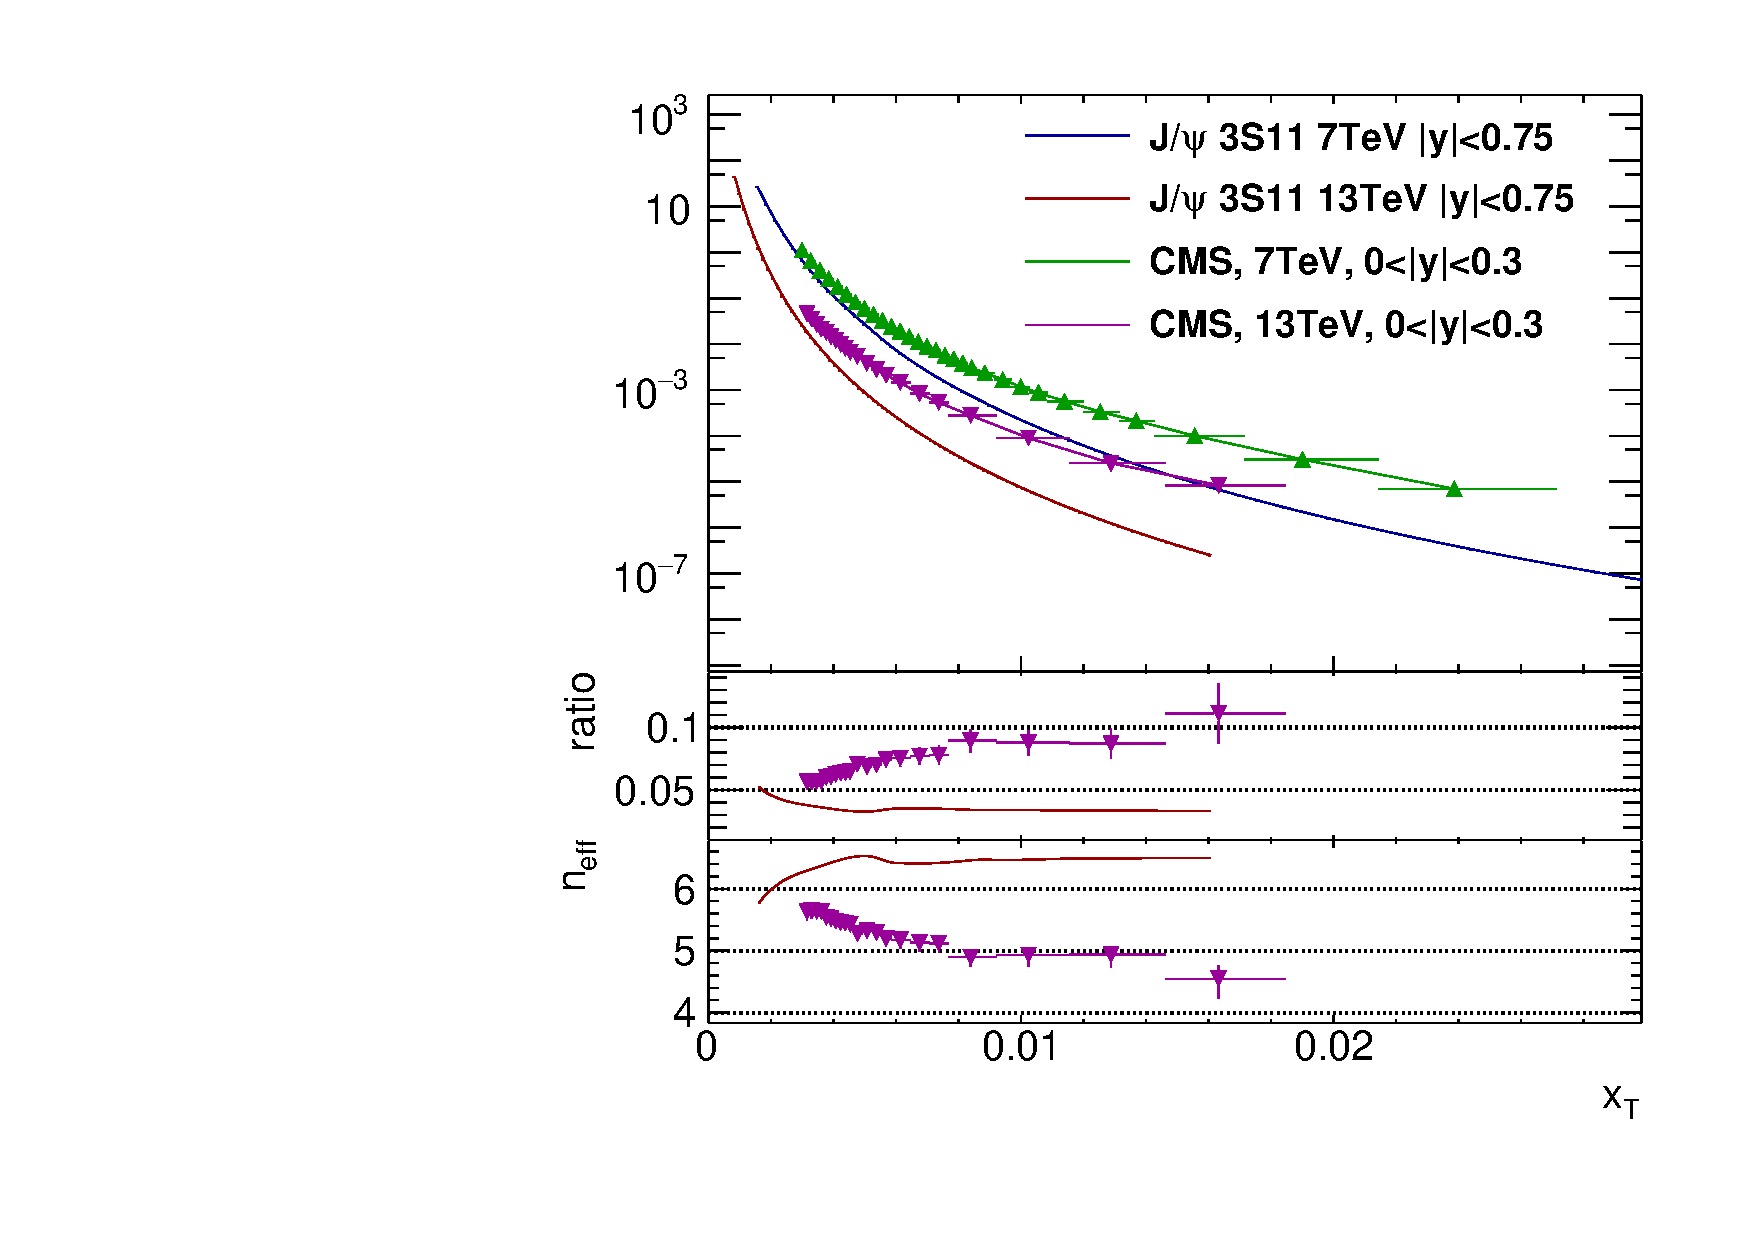
\includegraphics[width=0.49\textwidth]{theory_3S11_midrap.pdf}
   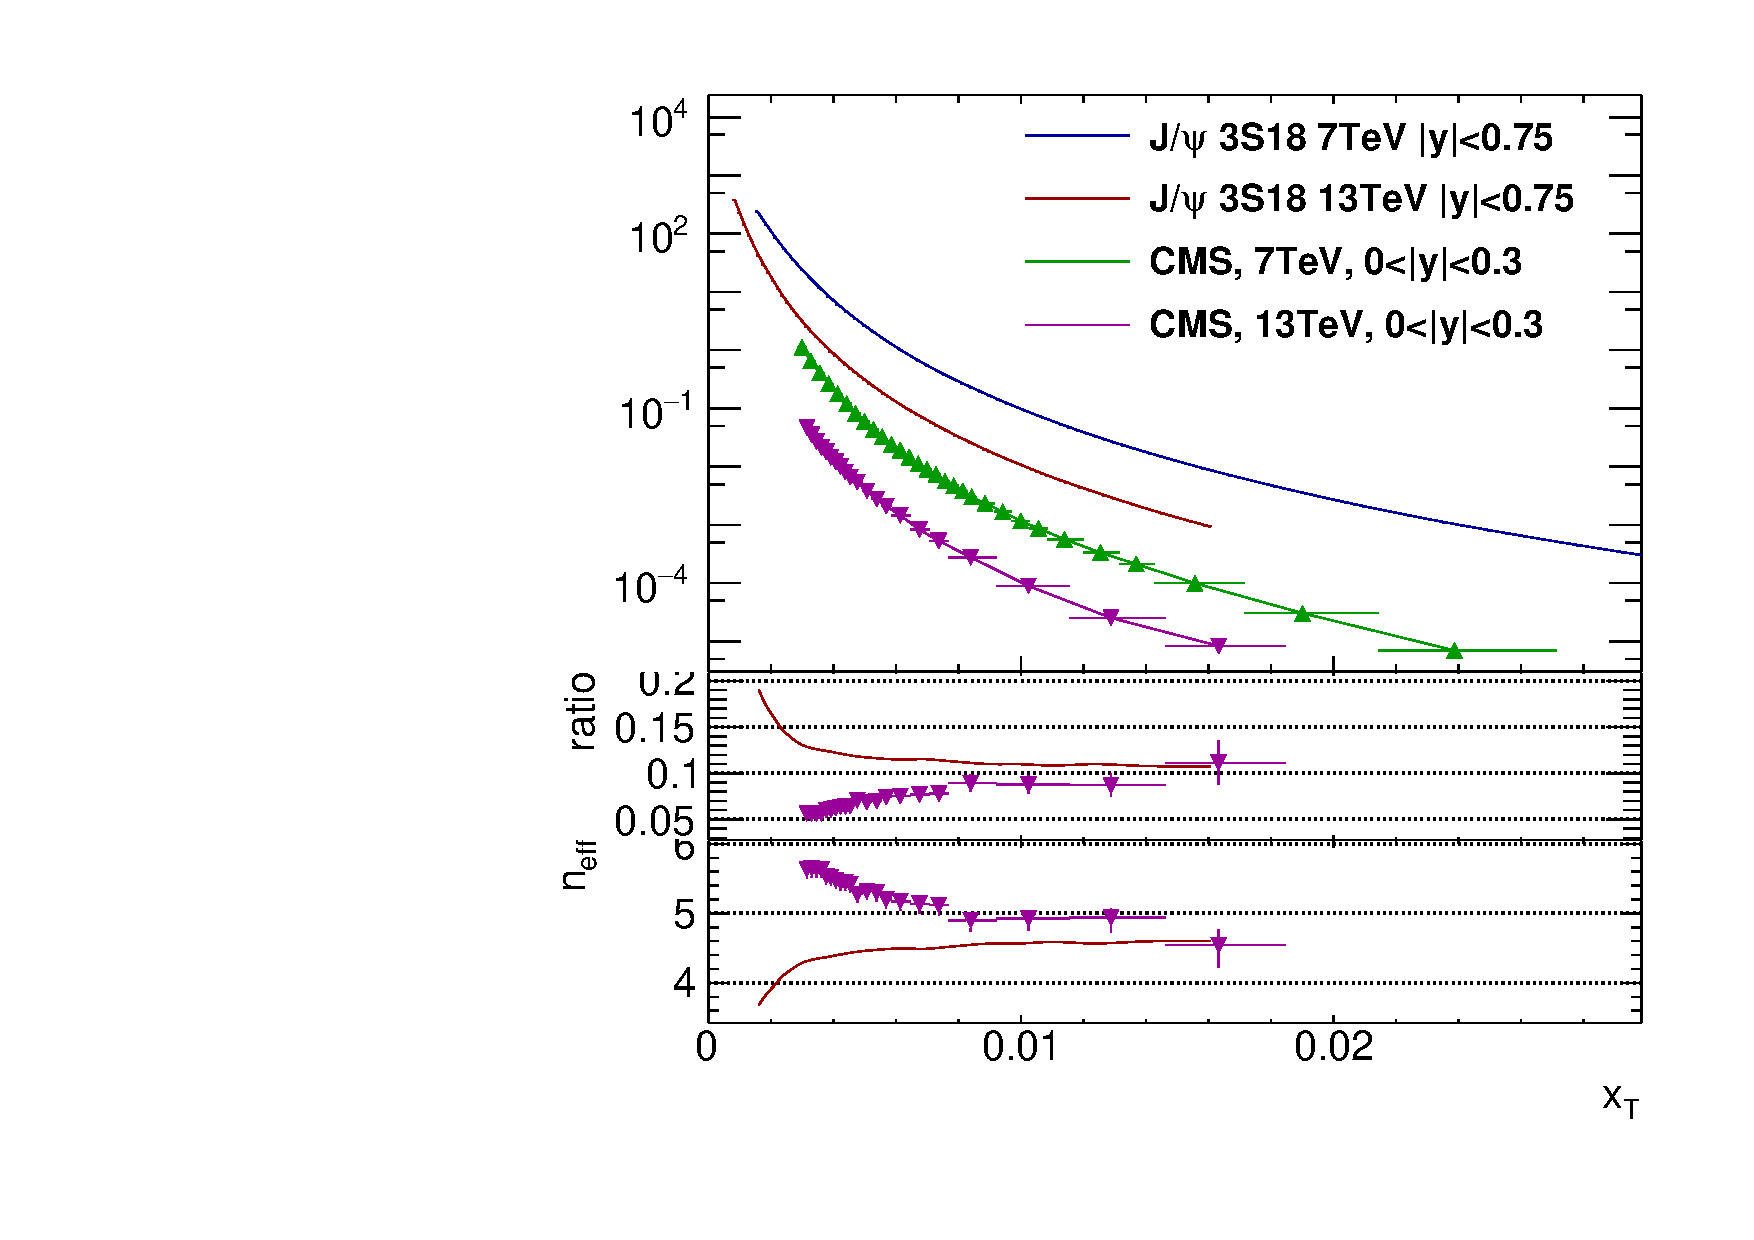
\includegraphics[width=0.49\textwidth]{theory_3S18_midrap.pdf}
   
   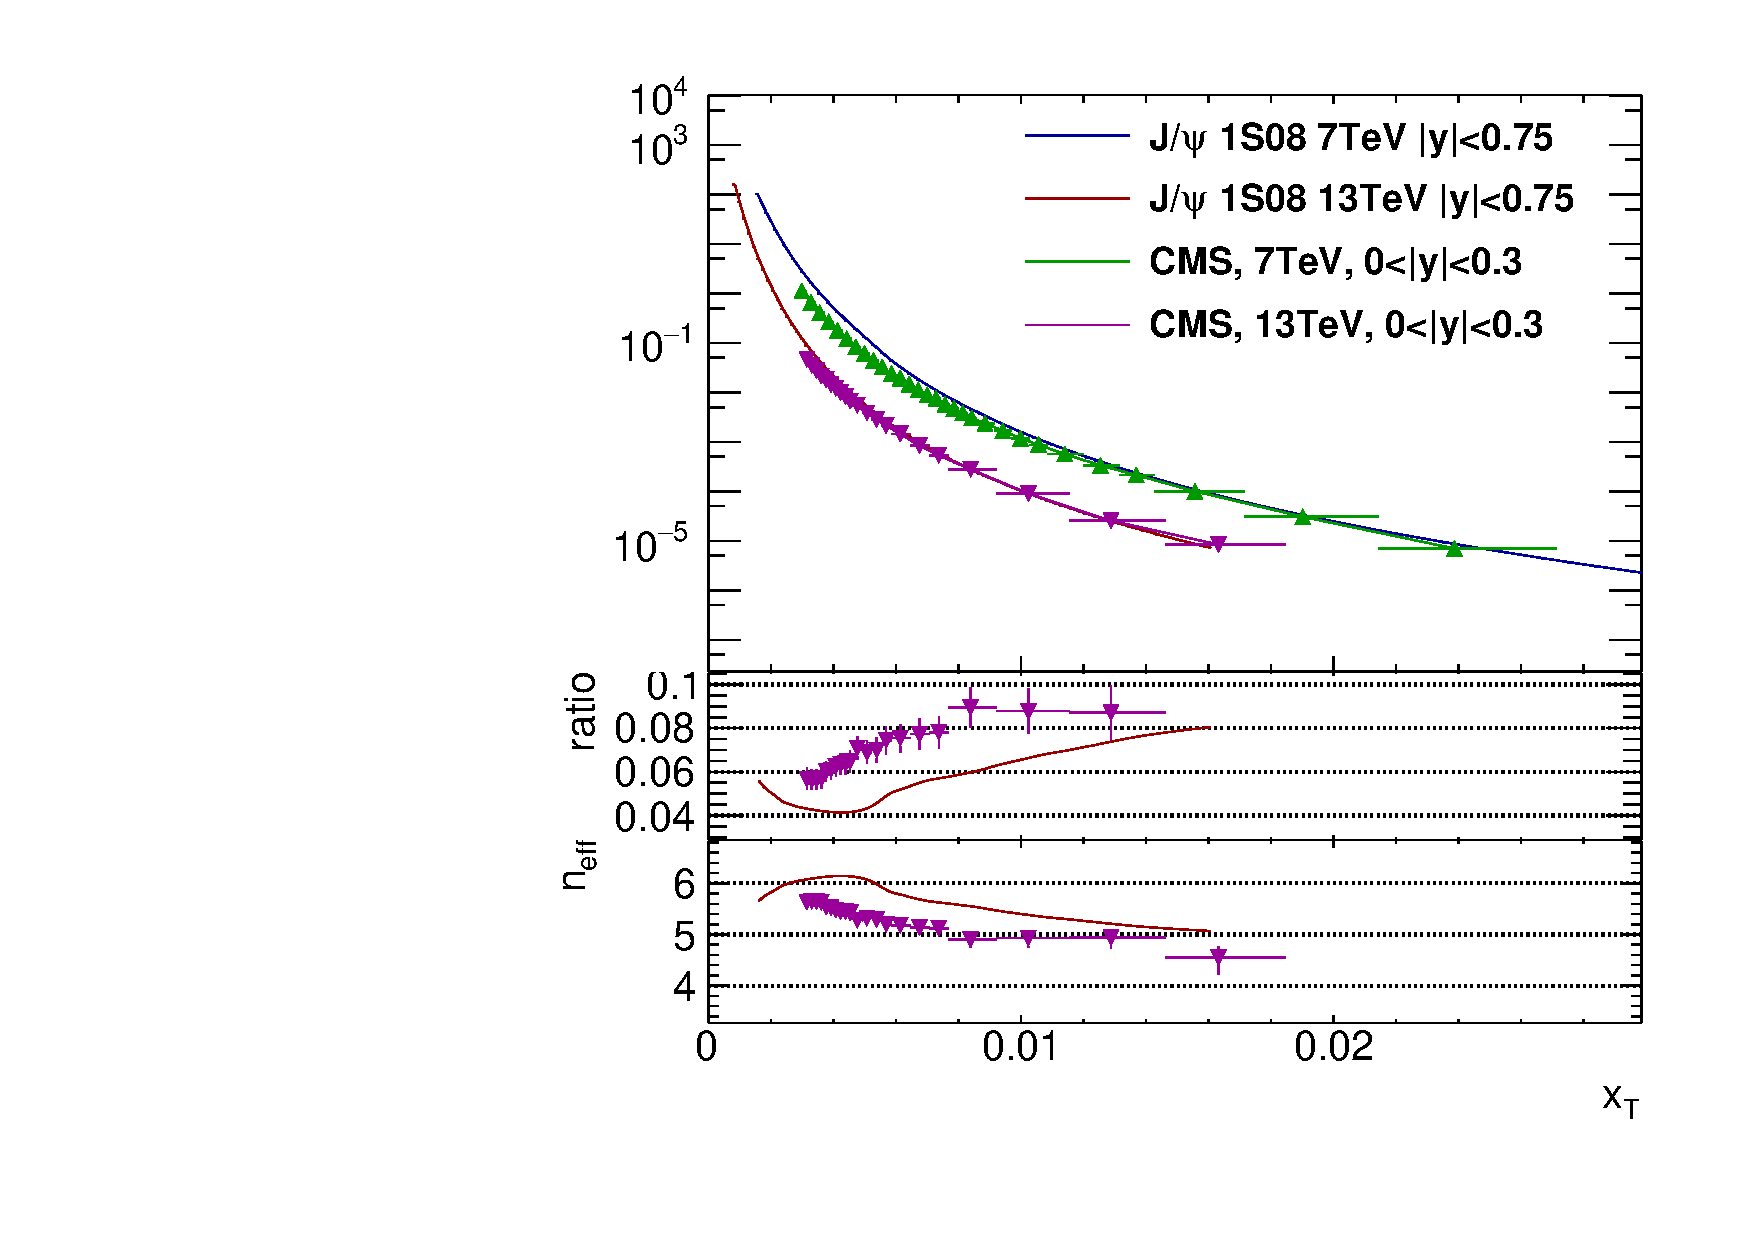
\includegraphics[width=0.49\textwidth]{theory_1s08_midrap.pdf}
   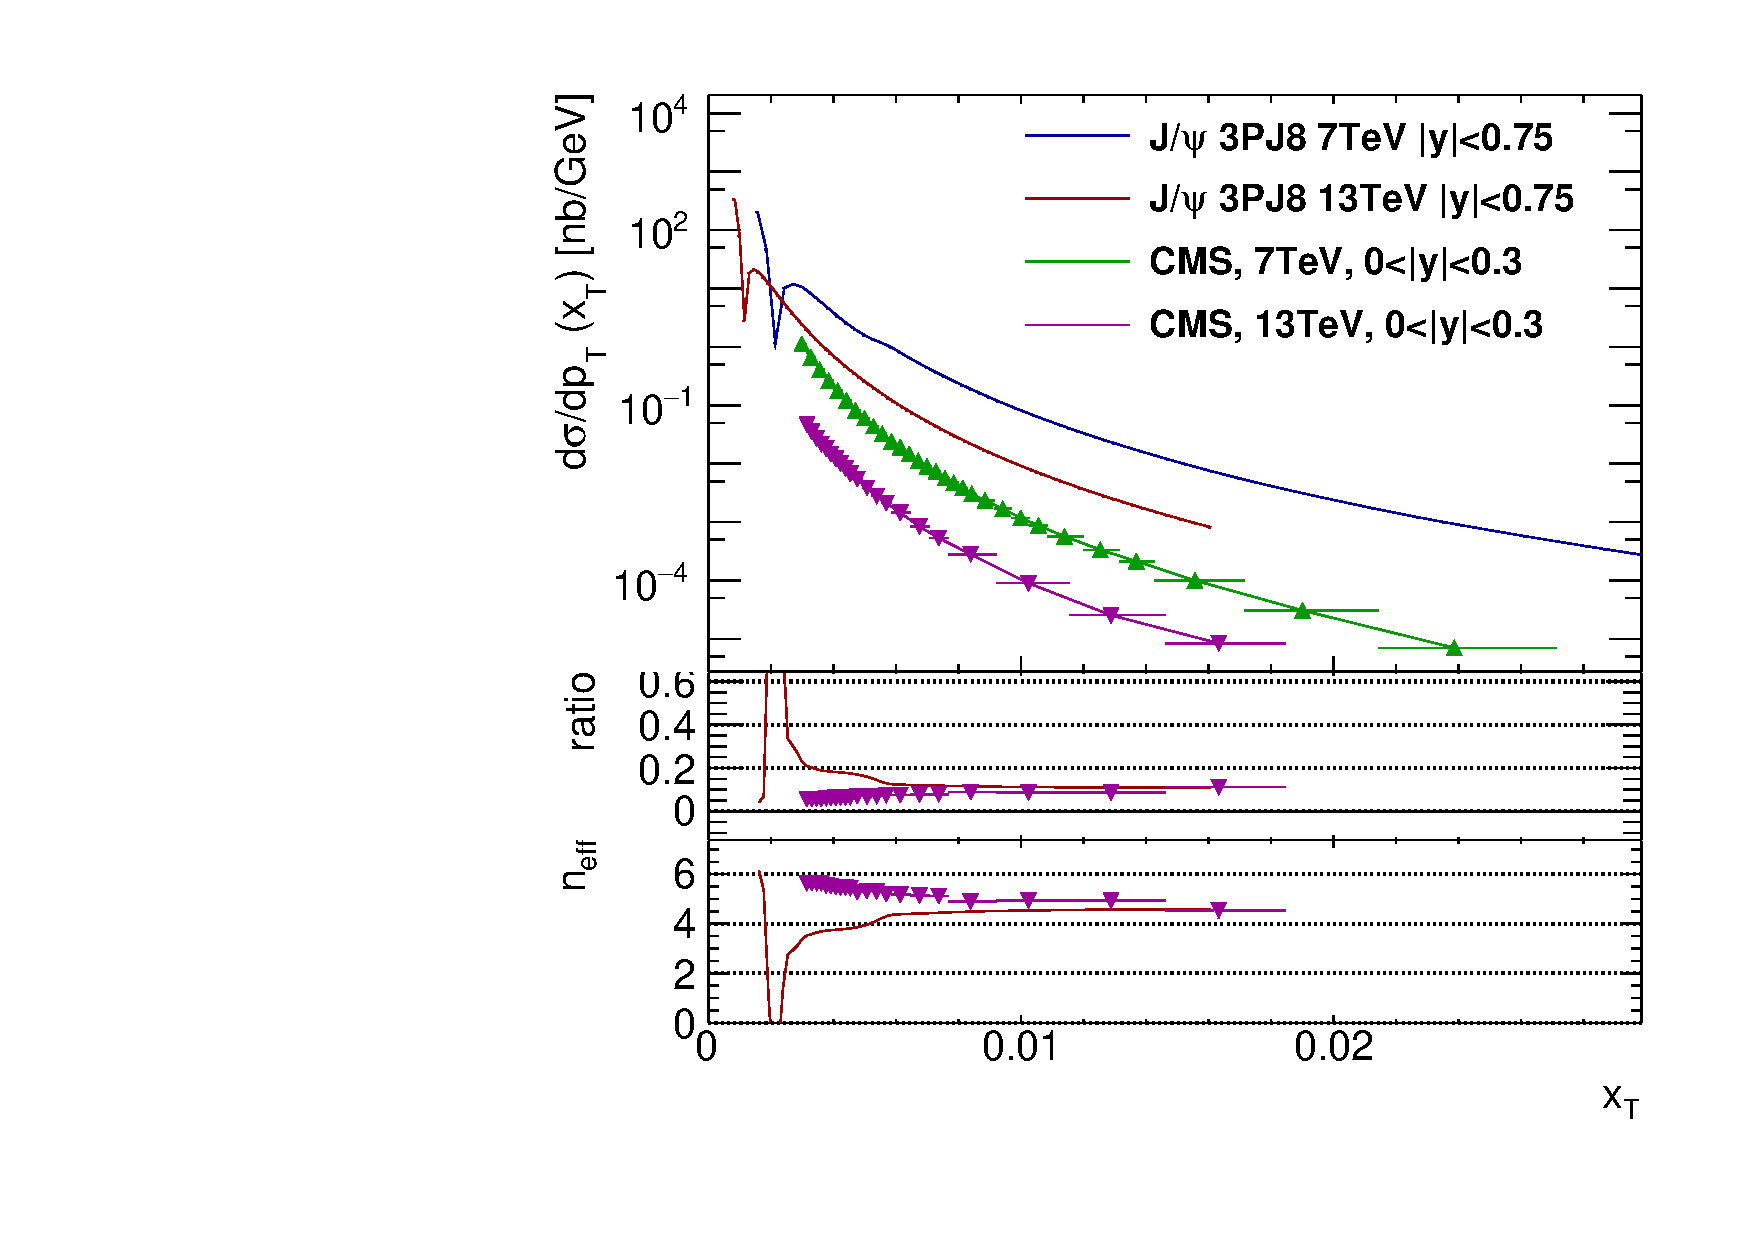
\includegraphics[width=0.49\textwidth]{theory_3PJ8_midrap.pdf}
  \end{center}

 \end{figure}


 \begin{thebibliography}{9}
 \bibitem{xt} F.~Arleo, S.~J.~Brodsky, D.~S.~Hwang and A.~M.~Sickles,
  %``Higher-Twist Dynamics in Large Transverse Momentum Hadron Production,''
  Phys.\ Rev.\ Lett.\  {\bf 105} (2010) 062002.
%   doi:10.1103/PhysRevLett.105.062002
%   [arXiv:0911.4604 [hep-ph]].
  %%CITATION = doi:10.1103/PhysRevLett.105.062002;%%
  %55 citations counted in INSPIRE as of 09 Nov 2017
  \bibitem{lw}  G.~D.~Lafferty and T.~R.~Wyatt,
  %``Where to stick your data points: The treatment of measurements within wide bins,''
  Nucl.\ Instrum.\ Meth.\ A {\bf 355} (1995) 541.
%   doi:10.1016/0168-9002(94)01112-5
  %%CITATION = doi:10.1016/0168-9002(94)01112-5;%%
  %196 citations counted in INSPIRE as of 09 Nov 2017
  \bibitem{atlas78}
  G.~Aad {\it et al.} [ATLAS Collaboration],
  %``Measurement of the differential cross-sections of prompt and non-prompt production of $J/\psi $ and $\psi (2\mathrm {S})$ in $pp$ collisions at $\sqrt{s} = 7$ and 8 TeV with the ATLAS detector,''
  Eur.\ Phys.\ J.\ C {\bf 76} (2016) no.5,  283.
%   doi:10.1140/epjc/s10052-016-4050-8
%   [arXiv:1512.03657 [hep-ex]].
  %%CITATION = doi:10.1140/epjc/s10052-016-4050-8;%%
  %26 citations counted in INSPIRE as of 09 Nov 2017
  \bibitem{lhcb276}
  R.~Aaij {\it et al.} [LHCb Collaboration],
  %``Measurement of $J/\psi$ production in $pp$ collisions at $\sqrt{s}=2.76$ TeV,''
  JHEP {\bf 1302} (2013) 041.
%   doi:10.1007/JHEP02(2013)041
%   [arXiv:1212.1045 [hep-ex]].
  %%CITATION = doi:10.1007/JHEP02(2013)041;%%
  %60 citations counted in INSPIRE as of 09 Nov 2017
  \bibitem{lhcb7}
  R.~Aaij {\it et al.} [LHCb Collaboration],
  %``Measurement of $J/\psi$ production in $pp$ collisions at $\sqrt{s}=7~\rm{TeV}$,''
  Eur.\ Phys.\ J.\ C {\bf 71} (2011) 1645.
%   doi:10.1140/epjc/s10052-011-1645-y
%   [arXiv:1103.0423 [hep-ex]].
  %%CITATION = doi:10.1140/epjc/s10052-011-1645-y;%%
  %357 citations counted in INSPIRE as of 09 Nov 2017
  \bibitem{lhcb8}
  R.~Aaij {\it et al.} [LHCb Collaboration],
  %``Production of J/psi and Upsilon mesons in pp collisions at sqrt(s) = 8 TeV,''
  JHEP {\bf 1306} (2013) 064
  doi:10.1007/JHEP06(2013)064
  [arXiv:1304.6977 [hep-ex]].
  %%CITATION = doi:10.1007/JHEP06(2013)064;%%
  %102 citations counted in INSPIRE as of 09 Nov 2017
  \bibitem{lhcb13}
  R.~Aaij {\it et al.} [LHCb Collaboration],
  %``Measurement of forward $J/\psi$ production cross-sections in $pp$ collisions at $\sqrt{s}=13$ TeV,''
  JHEP {\bf 1510} (2015) 172
   Erratum: [JHEP {\bf 1705} (2017) 063].
%   doi:10.1007/JHEP05(2017)063, 10.1007/JHEP10(2015)172
%   [arXiv:1509.00771 [hep-ex]].
  %%CITATION = doi:10.1007/JHEP05(2017)063, 10.1007/JHEP10(2015)172;%%
  %61 citations counted in INSPIRE as of 09 Nov 2017
  \bibitem{cms7}
  V.~Khachatryan {\it et al.} [CMS Collaboration],
  %``Measurement of J/ψ and ψ(2S) Prompt Double-Differential Cross Sections in pp Collisions at $\sqrt{s}$=7  TeV,''
  Phys.\ Rev.\ Lett.\  {\bf 114} (2015) no.19,  191802.
%   doi:10.1103/PhysRevLett.114.191802
%   [arXiv:1502.04155 [hep-ex]].
  %%CITATION = doi:10.1103/PhysRevLett.114.191802;%%
  %47 citations counted in INSPIRE as of 09 Nov 2017
  \bibitem{cms13}
  A.~M.~Sirunyan {\it et al.} [CMS Collaboration],
  %``Measurement of quarkonium production cross sections in pp collisions at $\sqrt{s}=$ 13 TeV,''
  arXiv:1710.11002 [hep-ex].
  %%CITATION = ARXIV:1710.11002;%%
 \end{thebibliography}

\end{document}
